% Copyright 2014-2016, 2018-2019 Frédéric Vincent, Thibaut Paumard
%
% This file is part of Gyoto.
%
% Gyoto is free software: you can redistribute it and/or modify
% it under the terms of the GNU General Public License as published by
% the Free Software Foundation, either version 3 of the License, or
% (at your option) any later version.
%
% Gyoto is distributed in the hope that it will be useful,
% but WITHOUT ANY WARRANTY; without even the implied warranty of
% MERCHANTABILITY or FITNESS FOR A PARTICULAR PURPOSE.  See the
% GNU General Public License for more details.
%
% You should have received a copy of the GNU General Public License
% along with Gyoto.  If not, see <http://www.gnu.org/licenses/>.

\documentclass[a4paper,12pt]{article}

% The build system will provide this command to make out-of-tree build
% work
\providecommand{\GyotoSrcDir}{../..}

\usepackage[]{natbib}  

\usepackage{fullpage}

\usepackage{calc}
\usepackage[usenames,dvipsnames]{color}

\usepackage[latin1]{inputenc} 
\usepackage[T1]{fontenc}    
\usepackage{textcomp}
\usepackage{rotating}

\usepackage[frenchb,english]{babel} 
\usepackage{amssymb,amsmath} 
\usepackage{float}
\usepackage{hyperref}                
\usepackage{amstext}
\usepackage{tipa}
%\usepackage{palatino}
\usepackage{fancyvrb}
\DefineVerbatimEnvironment{code}{Verbatim}{fontsize=\small}
\newcommand{\D}{\mathrm{d}}  
\newcommand{\GYOTO}{\texttt{GYOTO}}
\newcommand{\Metric}{\texttt{Metric}}
\newcommand{\Astrobj}{\texttt{Astrobj}}
\newcommand{\Spectrum}{\texttt{Spectrum}}

\DeclareMathOperator{\sgn}{sgn}
\DeclareMathOperator{\atantwo}{atan2}
\DeclareMathOperator{\proj}{proj}

\graphicspath{{\GyotoSrcDir/doc/images/}}


\begin{document}

\begin{center}
\section*{\Huge{Quick User Guide for \texttt{GYOTO}}}

\vspace{0.5cm}

% Let's enter the date manually.  Need to update it at least for each
% release. Use git log to find out the last change to the user manual.
\Large{Updated September 5, 2019}
%\today

\vspace{4cm}

\begin{figure}[htbp]
\centering
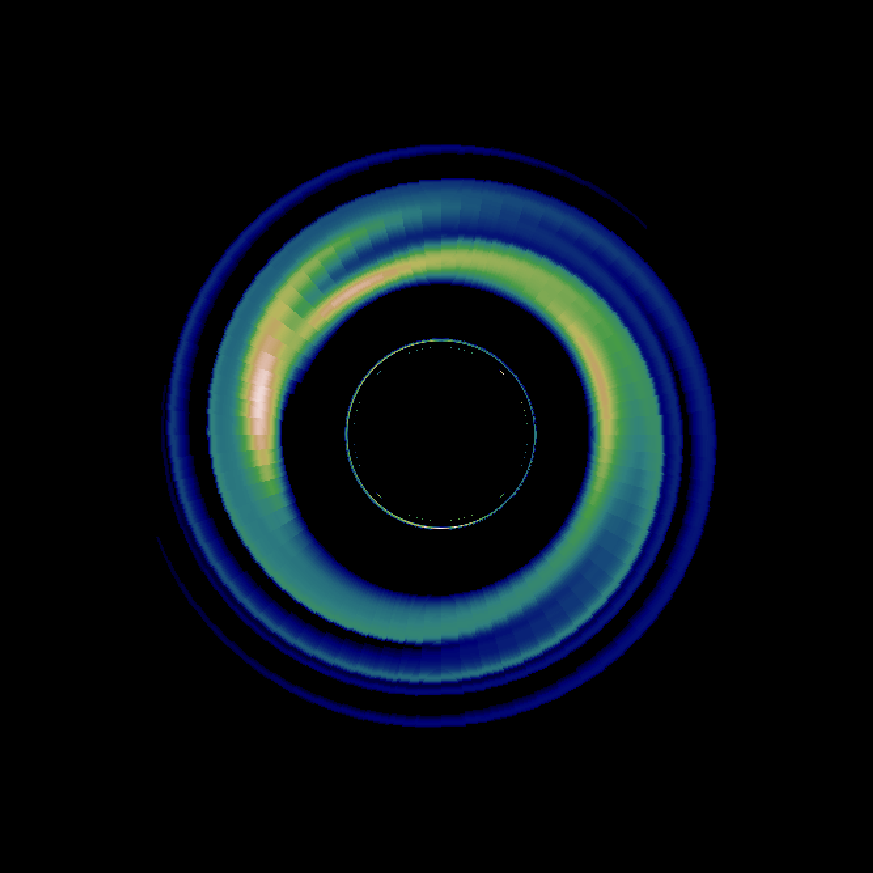
\includegraphics[width=10cm,height=10cm]{RWI_t1822_nu18.pdf}
%\caption{}
%\label{fig:hotspot}
\end{figure}

\end{center}



\newpage

\section*{Introduction - Scope of this Guide}



This Guide aims at giving a general presentation of the \textit{General relativitY Orbit Tracer of Observatoire de Paris}, \texttt{GYOTO} (pronounced \textipa{[dZIoto]}, as for the Italian trecento painter Giotto di Bondone). This text is not a lecture on ray-tracing techniques and is only devoted to presenting the code so that it can be quickly handled by any user. Readers interested in the physics behind \texttt{GYOTO} are referred to~\citet[][and references therein]{vincent11a,vincent12a}. The aim of this Guide is also to present the code in sufficient details so that people interested to develop their own version of \texttt{GYOTO} can do it easily.

\texttt{GYOTO} is an open source C++ code with a Yorick plug-in that computes null and time-like geodesics in the Kerr metric as well as in any metric computed within the framework of the 3+1 formalism of general relativity. This code allows to compute mainly images and spectra of astrophysical sources emitting electromagnetic radiation in the vicinity of compact objects (e.g. accretion disks or nearby stars). 

As \texttt{GYOTO} is continually evolving, this guide will (hopefully) be regularly updated to present the new functionalities added to the code. However, this guide does not constitute a full reference. The reference manual is built from the C++ header files using \texttt{doxygen} into the \texttt{doc/html/} directory of the source tree. It is also available online (rebuilt every night) at \url{http://gyoto.obspm.fr/}.

The reader is strongly encouraged to give feedback on this Manual, report typos, ask questions or suggest improvements by sending an email to \url{frederic.vincent@obspm.fr}

\tableofcontents



\newpage

\section{Installing \texttt{GYOTO}}
\label{install}

\texttt{GYOTO} is freely available at the URL \url{http://gyoto.obspm.fr/}. This URL hosts the online manual of \texttt{GYOTO}, with installation instructions and brief descriptions of the code architecture.

\texttt{GYOTO} is version-controlled with the \texttt{git} software that you should install on your machine.
Before uploading the code, be sure that the \texttt{xerces-c3} (or \texttt{xercesc3} depending on the
architecture) and \texttt{cfitsio} libraries are installed on your system: \texttt{GYOTO} won't compile without these.
It is also better (but not required) to install the \texttt{udunits2} library. Once this is done, just type on a command line
\begin{code}
git clone git://github.com/gyoto/Gyoto.git
\end{code}  
which will create a \texttt{Gyoto} repository. It contains directories \texttt{bin}, \texttt{lib}, \texttt{include}, \texttt{doc}, \texttt{yorick}
containing respectively the core code and executable, the \texttt{.C} source files, the \texttt{.h} headers, the documentation
and \texttt{Yorick} plug-in related code. 

In the \texttt{Gyoto} repository, use the standard 
\begin{code}
./configure; make; sudo make install 
\end{code}
commands
to build the code.

In case of problems, have a look at the \texttt{INSTALL} file that gives important complementary informations on how to install \texttt{GYOTO}.

\section{Basic usage}
\subsection{Using the \texttt{gyoto} command-line tool}
\label{demo}

The most basic way of using \texttt{GYOTO} is through the
\texttt{gyoto} command-line tools. It relies on two kinds of files: an
\texttt{XML} file containing the inputs and a \texttt{FITS} file
containing the outputs.

\subsubsection{XML input file}

You can find examples of \texttt{XML} input files in \texttt{doc/examples/}. Let us consider the computation of the image of a standard Page-Thorne accretion disk in Boyer-Lindquist coordinates, described in \texttt{example-page-thorne-disk-BL.xml}. 

\begin{sloppypar} %to allow proper newline for long words (in texttt)
If you are not familiar with \texttt{XML} language, just remember that an \texttt{XML} file is made of several fields beginning with the \texttt{<Field Name>} and ending with \texttt{</Field Name>}. One field can have sub-fields, defined with the same symbols. For instance in \texttt{example-page-thorne-disk-BL.xml}, there is one global field, \texttt{Scenery}, describing the scenery that will be ray-traced, with a few sub-fields: \texttt{Metric} describing the metric used for the computation, here the Kerr metric in Boyer-Lindquist coordinates; \texttt{Screen} describing the observer's screen properties; finally \texttt{Astrobj} describing the astrophysical object that will be ray-traced, here a Page-Thorne accretion disk.
All the parameters in this input file can be changed to specify a new scenery. 

Let us present in details the \texttt{example-page-thorne-disk-BL.xml} file:

\begin{code}
<?xml version="1.0" encoding="UTF-8" standalone="no"?>
<Scenery>
\end{code}

The following lines specify the metric: it is the Kerr metric, expressed in Boyer-Lindquist coordinates, with spin 0 (so the Schwarzschild metric here!):

\begin{code}
  <Metric kind = "KerrBL">
    <Spin>
      0.
    </Spin>
  </Metric>
\end{code}

The metric is now defined, let us describe the observer's screen.
The \texttt{Position} field gives the screen's 4-position 
in Boyer-Lindquist coordinates $(t,r,\theta,\varphi)$, 
angles in radians, time and radius in geometrical units  
(i.e. units with $c$ and $G$ put to 1). The \texttt{Time} field
gives the time of observation. The \texttt{FieldOfView} is given in radians.
The screen's \texttt{Resolution} is the number of screen pixels in each
direction.

\begin{code}
  <Screen>
    <Position>
      1000.
       100.
       1.22
       0.
    </Position>
    <Time unit="geometrical_time">
       1000.   
    </Time>
    <FieldOfView>
       0.314159265358979323846264338327950288419716
     </FieldOfView>
     <Resolution> 
       32   
     </Resolution>
  </Screen>
\end{code}

The screen is now defined. The following line describes the target object that will be ray-traced:

\begin{code}
   <Astrobj kind = "PageThorneDisk"/>
\end{code}

Here the target object is very simple and requires no specifications.
The \texttt{Scenery} is now fully defined and the field can be closed

\begin{code}
  </Scenery>
\end{code}

This is the end of the \texttt{XML} input file!

\end{sloppypar}

\subsubsection{Calling \texttt{gyoto}}


We will now use the \texttt{gyoto} command-line tools to ray-trace the
scenery described in this \texttt{XML} file. The command-line options
are documented in the usual UNIX-style manpage:
\begin{code}
  $ man gyoto
\end{code}
%$

Once the \texttt{XML} input file is ready, the call to \texttt{gyoto} is done according to the following line:
\begin{code}
 $ gyoto input.xml \!output.fits
\end{code}
%$
where \texttt{input.xml} is the above mentioned \texttt{XML} file and \texttt{output.fits} is the name of the \texttt{FITS} that will contain the result of the computation.
The \texttt{!} before the \texttt{.fits} file allows to overwrite a pre-existing file. If you remove it, an error will occur if the \texttt{.fits} file already exists. 

\begin{figure}
\centering
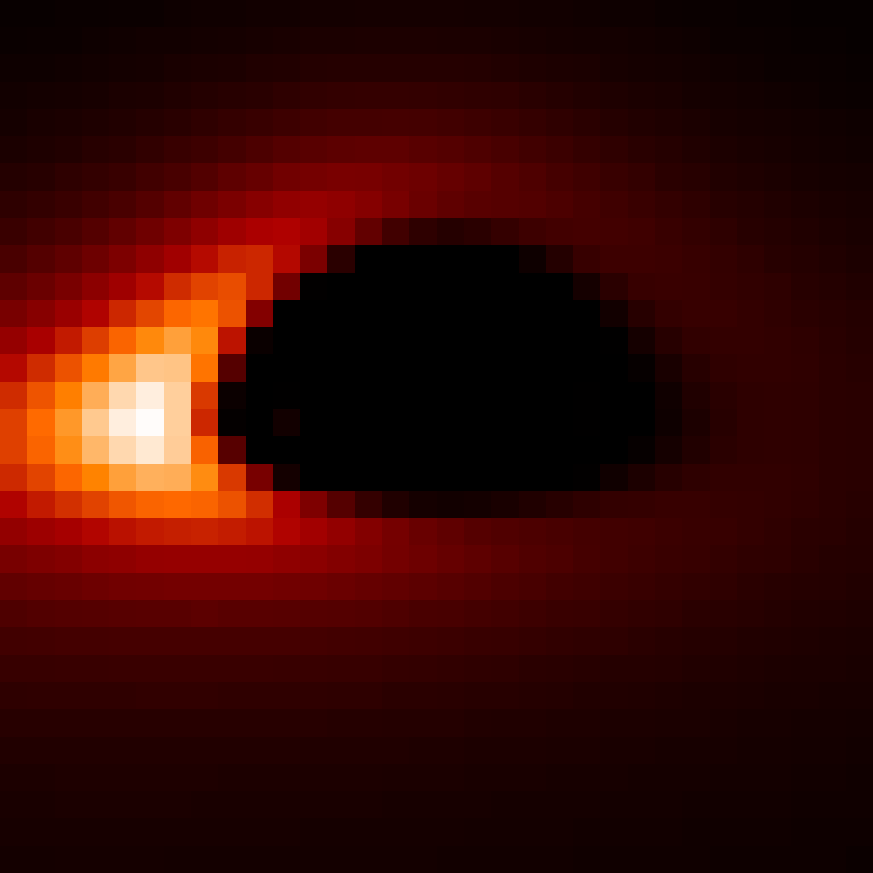
\includegraphics[width=8cm,height=8cm]{DemoPageThorne.pdf}
\caption{Image of a Page-Thorne thin accretion disk around a Schwarzschild black hole, with a $32\times 32$ pixels screen.}
\label{fig:demo}
\end{figure}
The line above asks \texttt{GYOTO} to integrate a null geodesic from each pixel of the screen backward in time towards the astrophysical object.
\subsubsection{FITS output file}

Once the computation is performed, the \texttt{output.fits} file is created. You can visualise it by using the \texttt{ds9} software (\url{http://hea-www.harvard.edu/RD/ds9/site/Home.html}) and simply running:

\begin{code}
 $ ds9 ouput.fits
\end{code}
%$

For instance, if you use the \texttt{example-page-thorne-disk-BL.xml} as is, you will obtain Fig.~\ref{fig:demo}.

\subsection{Parallelisation}

Ray-tracing of several hundreds of light-rays is a problem that is
easily parralelised, by letting different CPUs compute distinct
geodesics. \texttt{GYOTO} offers several facilities to perform such
parallelisation, depending on the hardware and software environment.

\subsubsection{Multi-threading}

You can accelerate computations by using several cores on a computer
using the \texttt{----nthreads=NCORES} option. \texttt{NCORES} is the
number of threads that \texttt{GYOTO} will use. The optimal value is
usually the number of hardware CPU cores on the machine. This option
can also be specified in the input file using the
\texttt{$<$NThreads$>$} entity. This facility does not work for
LORENE-based metrics (see Sect.~\ref{3+1}).

\subsubsection{Multi-processing}

\texttt{GYOTO} is able to use the Message Passing Interface (MPI) to
distribute the workload over many CPUs, possibly hosted on different
computers. YOu can activate it by specifying
\texttt{--nprocesses=NPROCS}. \texttt{NPROCS} is the number of helper
processes that \texttt{GYOTO} will spawn. This does not include the
main \texttt{GYOTO} process, which will act as a manager for the
helpers. This functionnality relies on Astrobj::fillElement() and
Metric::fillElement() being properly implemented, which is not always
the case for new classes. Also, classes that use supplemental data
(additional files referenced to in the XML file) do require that these
supplemental data be accessible to all the processes using the same
absolute path. Most notably, Lorene metrics require such data. Astrobj
classes such as the PatternDisk also require on-disk data.

\subsubsection{Poor-mans parallelisation}

Another cheap way of parallelising the computation is to call several
\texttt{gyoto} instances, running on different CPUs or even on
different machines, each instance computing only a portion of the
image. This sort of basic parrallelisation is, naturally, supported by
all the \texttt{GYOTO} metrics.

You can ask \texttt{GYOTO} to compute only a fraction of
the screen's pixels by running one of:
\begin{code}
 $ gyoto -iIMIN:IMAX:DI -jJMIN:JMAX:DJ input.xml \!output.fits
 $ gyoto --ispec=IMIN:IMAX:DI --jspec=JMIN:JMAX:DJ input.xml \!output.fits
 $ gyoto --imin=IMIN --imax=IMAX --jmin=JMIN --jmax=JMAX --di=DI --dj=DJ \
            input.xml \!output.fits
\end{code}
%$
where \texttt{IMIN}, \texttt{IMAX}, \texttt{JMIN}, \texttt{JMAX} are the extremal indices of the pixels that will be computed. \texttt{DI} and \texttt{DJ} are the step size in the $i$ and $j$ direction respictively. With the \texttt{-{}-ispec} or \texttt{-i} syntax, \texttt{IMAX} defaults to \texttt{IMIN} if there is no colon in the specification, and to the image resolution otherwise. For instance, to compute only the geodesic that hits the central pixel of a $32 \times 32$ screen, type one of:
\begin{code}
 $ gyoto -i16 -j16 input.xml \!output.fits
 $ gyoto --ispec=16 --jspec=16 input.xml \!output.fits
 $ gyoto --imin=16 --imax=16 --jmin=16 --jmax=16 input.xml \!output.fits
\end{code}
%$
To compute only the points with even $i$ and od $j$, use (for instance) one of:
\begin{code}
 $ gyoto -i2::2 -j::2 input.xml \!output.fits
 $ gyoto --ispec=2::2 --jspec=1::2 input.xml \!output.fits
 $ gyoto --imin=2 --di=2 --jmin=1 --dj=2 input.xml \!output.fits
\end{code}
%$
To compute only the lower-right quadrant of the image:
\begin{code}
 $ gyoto -i17: -j:16 input.xml \!output.fits
 $ gyoto --ispec=17: --jspec=:16 input.xml \!output.fits
 $ gyoto --imin=17 --jmax=16 input.xml \!output.fits
\end{code}
%$

How to recombine the several output files into a single FITS file is
left as an exercise to the reader. It is easily done using any
scientific interpreted language such as
Yorick\footnote{\url{http://dhmunro.github.io/yorick-doc/}} or
Python\footnote{\url{https://www.python.org/}}.

\subsection{The \texttt{gyotoy} interface}
\label{sect:gyotoy}

The second most basic tool provided by \texttt{GYOTO} is
\texttt{gyotoy} (Fig.~\ref{fig:gyotoy}). This is a graphical user
interface to visualize a single geodesic. See the \texttt{README} and
\texttt{INSTALL} files for the prerequisites. Once the installation is
complete, your launch gyotoy as:
\begin{code}
 $ gyotoy  
\end{code}
%$
or, from the \texttt{yorick/} sub-directory of the built source tree:
\begin{code}
 $ ./yorick -i gyotoy.i
\end{code}
%$
followed, on the Yorick prompt, by:
\begin{code}
 > gyotoy
\end{code}

\begin{figure}
  \centering
  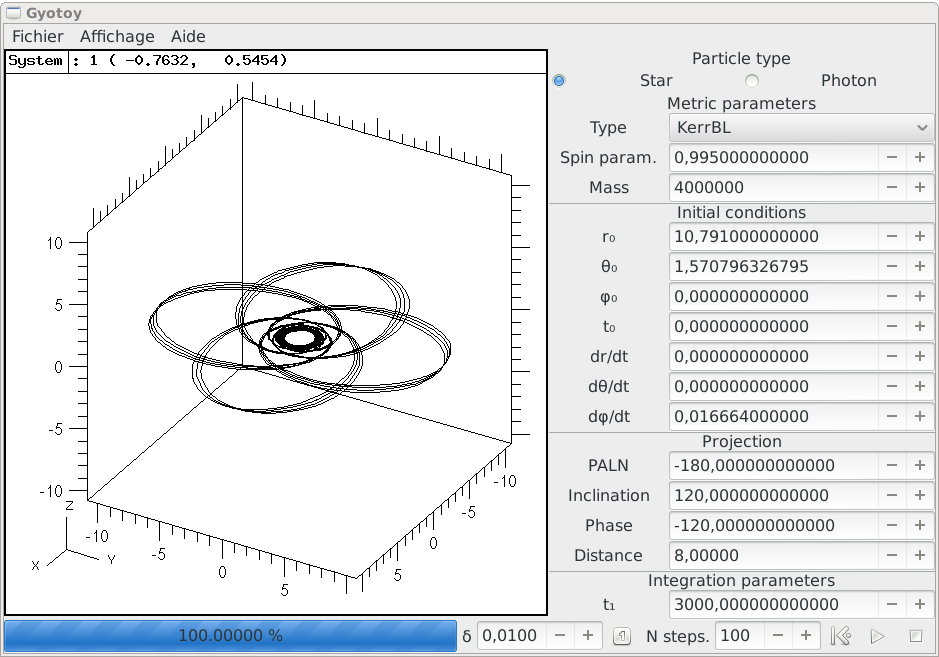
\includegraphics[width=0.7\linewidth]{gyotoy_screenshot.png}
  \caption{The \texttt{gyotoy} graphical user interface.}
  \label{fig:gyotoy}
\end{figure}
You can select a \texttt{KerrBL} metric and set the spin, or any other
metric defined in an \texttt{XML} file. As of writing, \texttt{gyotoy}
assumes that the coordinate system is spherical-like. It should work
in Cartesian coordinates as well, but the labels will be odd. It is
possible to select which kind of geodesic to compute (time-like or
light-like, using the \texttt{Star} or \texttt{Photon} radio buttons),
the initial position and 3-velocity of the particle, and the
projection (a.k.a. the position of the observer). The bottom tool bar
allows selecting a few numerical parameters such as whether or not to
use an adaptive step. Menus allow saving or opening the parameters as
an XML file, exporting the geodesic as a text file, and saving the
view as an image file in various formats. The view can be zoomed and
panned by clicking in the plot area.

\section{Beyond the basics: scripting \texttt{GYOTO}}

We have seen the two most basic ways of using \texttt{GYOTO}:
computing a single frame using the \texttt{gyoto} command-line tool,
and exploring a single geodesic using the \texttt{gyotoy}
interface. There is much more that \texttt{GYOTO} can be used for:
computing spectra, performing model-fitting, computing movies,
evaluating lensing effects etc.

\subsection{Using the Python module}
\label{sect:python}

The Python module is constantly evolving and some details can change
in future releases. It is documented in a Pythonic way, so
help(object) is your friend.

The Python module is split into several submodules:
\begin{description}
\item[gyoto.core] expose the generic framework compiled in
  \texttt{libgyoto};
\item[gyoto.std] expose the derived classes compiled in the
  standard plug-in, \texttt{libgyoto-stdplug};
\item[gyoto.lorene] expose the derived classes compiled in
  the Lorene plug-in, \texttt{libgyoto-lorene};
\item[gyoto.metric, gyoto.astrobj, gyoto.spectrometer, gyoto.spectrum]
  regroup the various Metrics, Astrobjs, etc. from the various
  extensions;
\item[gyoto.util] contains a few high-level wrappers and helper
  functions;
\item[gyoto.animate] contains a frame-work for producing videos based
  on Gyoto.
\end{description}

\subsubsection{Building and installing}

How to build and install these extensions is documented in INSTALL. At
the moment, this is not done automatically. The requisites are:
\begin{itemize}
\item Python (we use on recent Python 3, we support older releases
  down to Python 2.7 on a best effot basis), including the development
  files;
\item Swig (tested with 2.0.12 and 3.0.2);
\item NumPy, installed with its development files for the specific
  Python interpreter you plan on using.
\end{itemize}
For instance, on Debian Buster, to use compile the \texttt{gyoto}
extension for Python 3.7, you need the packages:
\begin{itemize}
\item \texttt{python3.7-dev};
\item \texttt{python3-numpy};
\item \texttt{swig} or \texttt{swig2.0}.
\end{itemize}
Configure the Gyoto source tree specifying the Python interpreter (if
you don't want to use the default on your system), build and install
gyoto, then move to the \texttt{python/} subdirectory, build and install:
\begin{code}
 $ ./configure PYTHON=/usr/bin/python3.7
 $ make
 $ sudo make install
 $ cd python
 $ make
 $ sudo make install
\end{code}
Depending on your system, you may need to add the directory where the
\texttt{gyoto/} directory containing \texttt{\_\_init\_\_.py} has been
installed to your PYTHONPATH variable.

\subsubsection{Using}

Some sample code can be found in \texttt{python/example.py}. The
Python extension matches the C++ API very closely, so the C++
reference in \texttt{doc/html/} is quite relevant. Most of it can also
be accessed through the Python function '\texttt{help}'.

The \texttt{gyoto.core} module should be enough to perform ray-tracing
on anykind of objects, even located in plug-ins:

Importing \texttt{gyoto}, \texttt{gyoto.core} or \texttt{gyoto.std}
would normally load the standard plug-in for you, but this is how you
would do it manually:
\begin{code}
  import gyoto.core
  gyoto.core.requirePlugin("stdplug")
\end{code}
Get help on Gyoto:
\begin{code}
  help(gyoto.core)
\end{code}
Read scenery from XML:
\begin{code}
  a=gyoto.core.Factory("../doc/examples/example-moving-star.xml")
  sc=a.scenery()
\end{code}
or:
\begin{code}
  import gyoto.util
  sc=gyoto.util.readScenery("../doc/examples/example-moving-star.xml")
\end{code}

Create Astrobj by name, access property by name:
\begin{code}
  tr=gyoto.core.Astrobj('Torus')
  tr.set('SmallRadius', 0.5)
\end{code}

To access methods of specific derived classes (for instance the Star
API, which allows computing time-like geodesics), the python extension
for a specific Gyoto plug-in must be imported:
\begin{code}
  from gyoto import std
  st=std.Star()
\end{code}
The various submodules and extensions are fully compatible with each
other:
\begin{code}
  sc=gyoto.core.Scenery()
  st=std.Star()
  sc.astrobj(st)
\end{code}
Pointers to the base classes can be up-cast to derived classes:
\begin{code}
  ao = sc.astrobj() # ao contains a Gyoto::Astrobj::Generic * pointer
  st = std.Star(ao) # if conversion fails, error is thrown
\end{code}

The source directory contains several examples and test cases. The
Python source for gyoto.util and gyoto.animate also provide rich
examples, always more up-to-date than the present documentation.

\subsection{Using the Yorick plug-in}
\label{sect:yorick}
Warning: the Yorick plug-in will not be udated with new features
anymore and we plan on phasing it out has soon as gyotoy has been
ported to Python. If in doubt, use Python instead.

Yorick is a fairly easy to learn interpreted computer language. We
provide a Yorick plug-in which exposes the \texttt{GYOTO}
functionalities to this language. This plug-in is self documented: at
the Yorick prompt, try:
\begin{code}
 > #include "gyoto.i"
 > help, gyoto
\end{code}

A lot of the \texttt{GYOTO} test suite is written in Yorick, which
provides many example code in the various \texttt{*.i} files in the
\texttt{yorick/} directory of the \texttt{GYOTO} source tree. Another
example is provided by the \texttt{gyotoy} graphical interface
(Sect.~\ref{sect:gyotoy}).

For Yorick basics, see:
\begin{itemize}
\item \url{https://github.com/dhmunro/yorick};
\item \url{http://dhmunro.github.io/yorick-doc/};
\item \url{http://yorick.sourceforge.net/};
\item \url{http://www.maumae.net/yorick/doc/index.php}.
\end{itemize}

As a very minimalist example, here is how to ray-trace an XML
scenery into a FITS file in Yorick:
\begin{code}
 $ rlwrap yorick
\end{code}
%$
This launches Yorick within the line-editing facility \texttt{rlwrap}
(provided separately). Then, from the Yorick prompt:
\begin{code}
 > #include "gyoto.i"
 > restore, gyoto;
 > sc = Scenery("input.xml");
 > data = sc(,,"Intensity");
 > fits_write, "output.fits", data;
\end{code}
or, in two lines:
\begin{code}
 > #include "gyoto.i"
 > fits_write, "output.fits", gyoto.Scenery("input.xml")(,,"Intensity");
\end{code}
Likewise, to integrate the spectrum over the field-of-view:
\begin{code}
 > #include "gyoto.i"
 > restore, gyoto;
 > sc = Scenery("input.xml");
 > data = sc(,,"Spectrum[mJy.pix-2]");
 > spectrum = data(sum, sum, );
 > freq = sc(screen=)(spectro=)(midpoints=, unit="Hz");
 > plg, spectrum, freq;
 > xytitles, "Frequency [Hz]", "Spectrum [mJy]";
\end{code}

MPI multi-processing is also available from within Yorick. To activate
this functionality, you must call \texttt{gyoto.mpiInit} early in your
script. Spawn the required number of processes using the
\texttt{mpispawn} method, and don't forget to use the
\texttt{mpiclone} method. Although not strictly necessary, it is also
recommended to explicitely terminate helper processes that have been
spawned in the background (using \texttt{mpispawn=0}, and to call
\texttt{gyoto.mpiFinalize} at the very end of your script:
\begin{code}
 > #include "gyoto.i"
 > restore, gyoto;
 > // call MPI_Init():
 > mpiInit;
 > sc = Scenery("input.xml");
 > // spawn helpers and send them the scenery
 > sc, mpispawn=12, mpiclone=;
 > // compute stuff
 > data =sc();
 > // shut down the helper processes
 > sc, mpispawn=0;
 > // shut down MPI
 > mpiFinalize;
 > quit;
\end{code}

The Yorick plug-in is not generated automatically. Therefore only a
subset of the Gyoto API is exposed. However, all the properties of any
object (most of what can be set in XML) can be read and written from
Yorick, with the possibility of specifying a unit for properties that
support it:
\begin{code}
 > #include "gyoto.i"
 > restore, gyoto;
 > tr = Astrobj("Torus");
 > noop, tr.SmallRadius(0.5, unit="geometrical");
 > small_radius_in_meters=tr.SmallRadius(unit="m");
 > tr, SmallRadius=0.5, unit="geometrical", LargeRadius=5e6, unit="m";
 > large_radius_in_default_unit=tr(LargeRadius=);
\end{code}


\subsection{Other languages}
\label{sect:swig}

The Python extension (Sect.~\ref{sect:python}) is generated
automatically using the Swig tool, with only little python-specific
code. It should therefore be rather easy to compile extensions for the
other languages that Swig supports (Tcl, java, R, and many others). If
you want it to happen, feel free to contact the Gyoto developers.

\subsection{Interfacing directly to the \texttt{GYOTO} library}

The core functionality is provided as a C++ shared library, which is
used both by the \texttt{gyoto} command-line tool and the Yorick
plug-in. You can, of course, interface directly to this library. The
reference is generated from the source code using \texttt{doxygen} in
the directory \texttt{doc/html/}. The application binary interface
(ABI) is likely to change with every commit. We try to maintain a
certain stability in the application programming interface (API), and
to maintain a stable branch whic honly sees bug-fixes between official
releases. But the effort we put into this stability is function of the
needs of our users. If you start depending on the \texttt{GYOTO}
library, please contact us (\texttt{gyoto@sympa.obspm.fr}): we will
try harder to facilitate your work, or at least warn you when there is
a significant API change.

\section{Choosing the right integrator}
\label{tuning}

Numerical ray-tracing can be very much time-consuming. In order to
control the numerical errors in your application, it is wise to
experiment with the numerical tuning parameters. \texttt{GYOTO}
provides several distinct integrators (depending on compile-time
options):
\begin{itemize}
\item the \texttt{Legacy} integrator, the first to have been introduced;
\item Boost\footnote{\url{http://www.boost.org/}} integrators from the
  \texttt{odeint}\footnote{\url{http://www.boost.org/doc/libs/1_55_0/libs/numeric/odeint/doc/html/index.html}}
  library. In \texttt{GYOTO}, they are called
  \texttt{runge\_kutta\_*} (see below).
\end{itemize}

The integrator and its numerical tuning parameters can be specified in
either of these three XML sections:
\begin{description}
\item[\texttt{Scenery}] to specify the integrator and parameters used
  during ray-tracing by the individual photons;
\item[\texttt{Photon}] if the XML file describes a single photon (the
  Yorick plug-in and the \texttt{gyotoy} tool can make use of such an
  XML file);
\item[\texttt{Astrobj}] if it is a \texttt{Star}, for specifying the
  integrator and parameters used to compute the orbit of this star.
\end{description}

The full set of tuning parameters that \emph{may be} supported by the
\texttt{Scenery} section is:
\begin{code}
<Scenery>
  <Integrator> runge_kutta_fehlberg78 </Integrator>
  <AbsTol> 1e-6 </AbsTol>
  <RelTol> 1e-6 </RelTol>
  <DeltaMax> 1.79769e+308 </DeltaMax>
  <DeltaMin> 2.22507e-308 </DeltaMin>
  <DeltaMaxOverR> 1.79769e+308 </DeltaMaxOverR>
  <MaxIter> 100000 </MaxIter>
  <Adaptive/>
  <Delta unit="geometrical"> 1 </Delta>
  <MinimumTime unit="geometrical_time"> -1.7e308 </MinimumTime>
</Scenery>
\end{code}

\begin{description}
\item[Integrator] the integrator to use (one of the runge\_kutta\_* or
  Legacy; default: if compiled-in, \texttt{runge\_kutta\_fehlberg78});
\item[AbsTol]\footnote{\label{note:abstol}The \texttt{Legacy}
    integrator does not support the AbsTol nor the RelTol parameters}
  absolute tolerance for adapting the integration step (see
  \url{http://www.boost.org/doc/libs/1_55_0/libs/numeric/odeint/doc/html/boost_numeric_odeint/odeint_in_detail/generation_functions.html});
\item[RelTol]\footnotemark[\value{footnote}] relative tolerance for
  adapting the integration step (idem);
\item[DeltaMax]\footnote{The \texttt{Legacy} integrator take the
    DeltaMin, DeltaMax and DeltaMaxOverR parameters in the
    \texttt{Metric} section.} the absolute maximum value for the
  integration step (defaults to the largest possible non-infinite
  value);
\item[DeltaMin]\footnotemark[\value{footnote}] the absolute minimum value (defaults to the smallest
  possible strictly positive value);
\item[DeltaMaxOverR]\footnotemark[\value{footnote}] this is $h=\delta_\text{max}/r$ such that, at any
  position, the integration step may not be larger than $h\times\;r$
  where $r$ is the current distance to the centre of the coordinate
  system (defaults to $1$).
\item[MaxIter] maximum number of integration steps (per photon);
\item[Adaptive] (or NonAdaptive) whether or not to use an adaptive step;
\item[Delta] integration step, initial in case it is adaptive. Not
  very important, but should be commensurable with the distance to the
  \texttt{Screen} (i.e. don't use Delta$=10^{-6}$ if the screen is at
  $10^{13}$ geometrical units!). Delta can be specified in any
  distance-like or time-like unit.
\item[MinimumTime] stop integration when the photon travels back to
  this date. Defaults to the earliest possible date. Can be specified
  in any time-like or distance-like unit.
\end{description}

\subsection{The Boost integrators}

If \texttt{GYOTO} was compiled with a C++11-capable compiler and with
the Boost library (version 1.53 or above), then the following
integrators are available:
\begin{itemize}
\item \texttt{runge\_kutta\_cash\_karp54};
\item \texttt{runge\_kutta\_fehlberg78};
\item \texttt{runge\_kutta\_dopri5};
\item \texttt{runge\_kutta\_cash\_karp54\_classic} (alternate
  implementation of\\ \texttt{runge\_kutta\_cash\_karp54}).
\end{itemize}

Those integrators are implemented in the \texttt{Worldline}
object. This has the advantage that, when ray-tracing the image of a
moving star (\texttt{Star} class), the star can use a different
integrator than the photons. These integrators support all of the
parameters described above.


\subsection{The \texttt{Legacy} integrator}

The \texttt{Legacy} integrator is a home-brewed
4\textsuperscript{th}-order, adaptive-step Runge--Kutta integrator. It
is always available, independent of any compile-time options. It does
not support AbsTol nor RelTol, and takes DeltaMin, DeltaMax and
DeltaMaxOver in the \texttt{Metric} section, not in the
\texttt{Scenery} or \texttt{Astrobj} section. It is not possible to
use different tuning parameters for the Star and the Photons if both
use the \texttt{Legacy} integrator.

The \texttt{Legacy} integrator is implemented in the \texttt{Metric}
object and may be re-implemented by specific \texttt{Metric}
kinds. Most notably, the \texttt{KerrBL} metric reimplements it (this
specific implementation takes advantage of the specific constants of
motion). When a metric reimplements the \texttt{Legacy} integrator, it
is possible to choose which implementation to choose by specifying
either \texttt{$<$GenericIntegrator$>$} or
\texttt{$<$SpecificIntegrator$>$} in the \texttt{$<$Metric$>$}
section. The \texttt{KerrBL} specific implementation of the
\texttt{Legacy} integrator accepts one additional tuning parameter:
\texttt{DiffTol}, which defaults to $10^{-2}$ and empirically seems to
have very little actual impact on the behaviour of the integrator.

\subsection{Integrator comparison}

\begin{figure}
  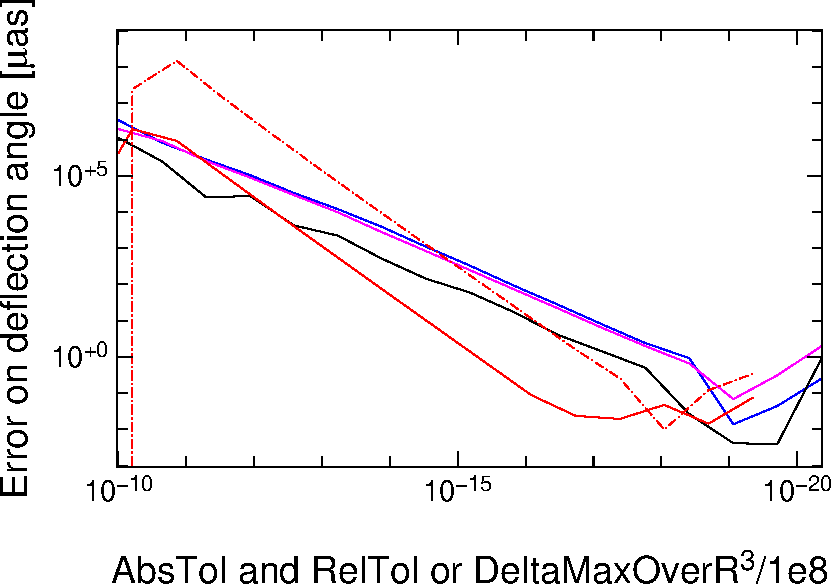
\includegraphics[width=0.32\textwidth]{doc-fig-dfl-tol.pdf}
  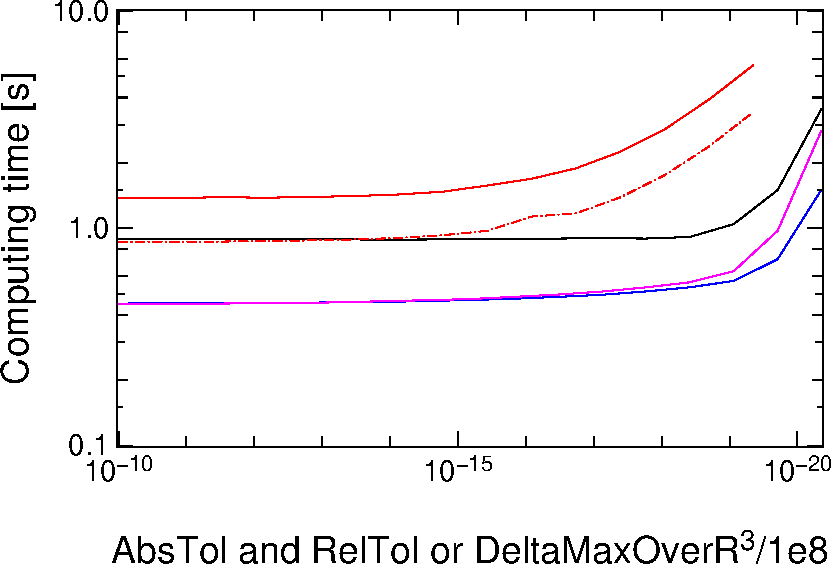
\includegraphics[width=0.32\textwidth]{doc-fig-ctime-tol.pdf}
  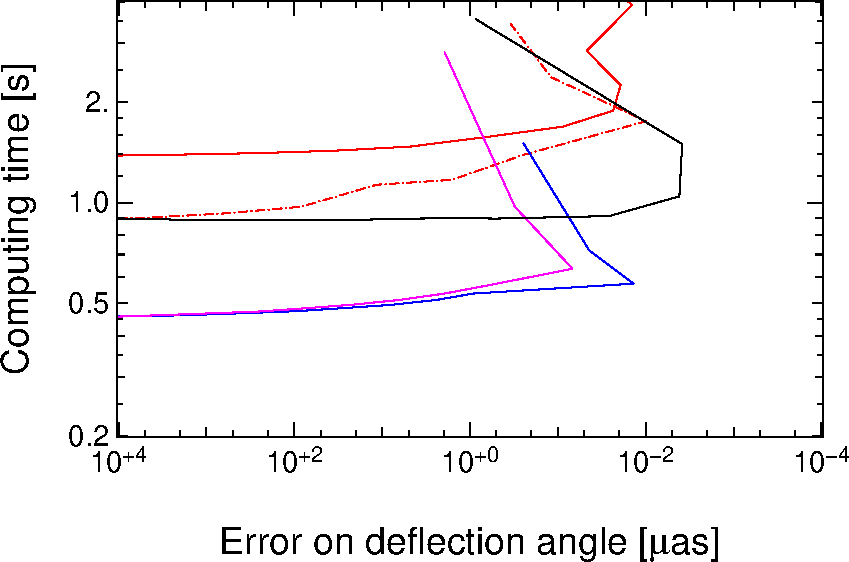
\includegraphics[width=0.32\textwidth]{doc-fig-dfl-ctime.pdf}
  \caption{Comparison of the integrators when measuring a deflection
    angle (see text). \emph{Left:} error on deflection angle
    vs. tuning parameter; \emph{centre:} computing time vs. tuning
    parameter; \emph{right:} computing time vs. error on deflection
    angle. Colours denote the integrator: \emph{red:} \texttt{Legacy}
    (\emph{solid:} specific \texttt{KerrBL} implementation,
    \emph{dash-dotted:} generic implementation); \emph{black:}
    \texttt{runge\_kutta\_fehlberg78}; \emph{blue:}
    \texttt{runge\_kutta\_karp54}; \emph{magenta:}
    \texttt{runge\_kutta\_dopri5}.}
\label{fig:integrators}
\end{figure}

It is advisable to try the various integrators in your context, and to
play with the tuning parameters. As a rule of thumbs, if you need to
change DeltaMin, DeltaMax, DeltaMaxOverR, or MaxIter, it probably
means that you should change for a higher-order integrator. The
highest order integrator is currently
\texttt{runge\_kutta\_fehlberg78} and is the default.

As an example, we have compared all the integrators for a simple
situation: the \texttt{Metric} is a Schwarzschild black-hole of
$4\times10^6\,M_\odot$, the \texttt{Screen} is at 8~kpc, a single
light-ray is launched $50\,\mu$as from the centre, we integrate the
light-ray (back in time) during twice the travel-time to the origin of
the coordinate centre and compute the deflection angle. We do that for
each integrator and a set of numerical tuning parameters. For the
\texttt{Legacy} integrator, we try both the generic integrator and the
specific \texttt{KerrBL} implementation, and use DeltaMaxOverR as
tuning parameter. For the Boost integrators, we use AbsTol and RelTol
as tuning parameters (they are kept equal to each-other). We then
compare the result for two values of the tuning parameter and measure
the computing time required for each
realisation.

For each integrator, there exists an optimum value or the tuning
parameter, for which the (estimated) uncertainty in deflection angle
is minimal (Fig.~\ref{fig:integrators}, left panel). As long as the
tuning parameter is larger than (or equal to) this optimum,
computation time varies very little (central panel). However, when the
tuning parameter becomes too small, numerical error and computation
time explode (right panel).

The two low-order Boost integrators are the fastest, the two
\texttt{Legacy} integrators are the slowest. The default,
\texttt{runge\_kutta\_fehlberg78}, has intermediate performance, but
seems to yield the smallest error and to be less sensitive on the
exact value of the tuning parameter close to its optimum.

All the integrators except the generic implementation of the
\texttt{Legacy} integrator agree to within $2\,\mu$as on the
deflection angle, which is of order 33°. The relative uncertainty is
therefore of order $10^{-11}$.

In conclusion, for this specific use case, the best choice seems to be:
\begin{code}
<Scenery>
 <Integrator>runge_kutta_fehlberg78</Integrator>
 <AbsTol>1e-19</AbsTol>
 <RelTol>1e-19</RelTol>
</Scenery>
\end{code}
If computation time is more critical than accuracy, the other Boost
integrators are also good choices.

The Yorick code that was used to generate Fig.~\ref{fig:integrators}
is provided in the \texttt{GYOTO} source code as
\texttt{yorick/compare-integrators.i}. You can run it from the top
directory of the built source tree as:
\begin{code}
  yorick/yorick -i yorick/compare-integrators.i
\end{code}

\section{\texttt{GYOTO} architecture}
\label{archi}

\subsection{\texttt{GYOTO} base classes}

\texttt{GYOTO} is basically organised around 8 base classes (see Fig.~\ref{fig:hierarch}):

\begin{itemize}
\item The \texttt{Metric} class: it describes the metric of the space-time (Kerr in Boyer-Lindquist coordinates, Kerr in Kerr-Schild coordinates, metric of a relativistic rotating star in 3+1 formalism...).
\item The \texttt{Astrobj} class: it describes the astrophysical target object that must ray-traced (e.g. a thin accretion disk, a thick 3D disk, a star...).
\item The \texttt{Spectrum} class: it describes the emitted spectrum of the \texttt{Astrobj}.
\item The \texttt{Worldline} class: it gives the evolving coordinates of a time-like or null geodesic. The \texttt{Star} class is a sub-class of \texttt{Worldline} as for the time being a star in \texttt{GYOTO} is only described by the time-like geodesic of its centre, with a given fixed radius.
\item The \texttt{WorldlineIntegState} class: it describes the integration of the \texttt{Worldline} in the given \texttt{Metric}.
\item The \texttt{Screen} class: it describes the observer's screen, its resolution, its position in space-time, its field of view.
\item The \texttt{Scenery} class: it describes the ray-tracing scene. It is made of a \texttt{Metric}, a \texttt{Screen}, an \texttt{Astrobj} and the quantities that must be computed (an image, a spectrum...).
\item The \texttt{Factory} class: it allows to translate the \texttt{XML} input file into C++ objects.
\end{itemize}

Fig.~\ref{fig:hierarch} presents the main \texttt{GYOTO} classes and their hierarchy.

\begin{figure}[htbp]
\centering
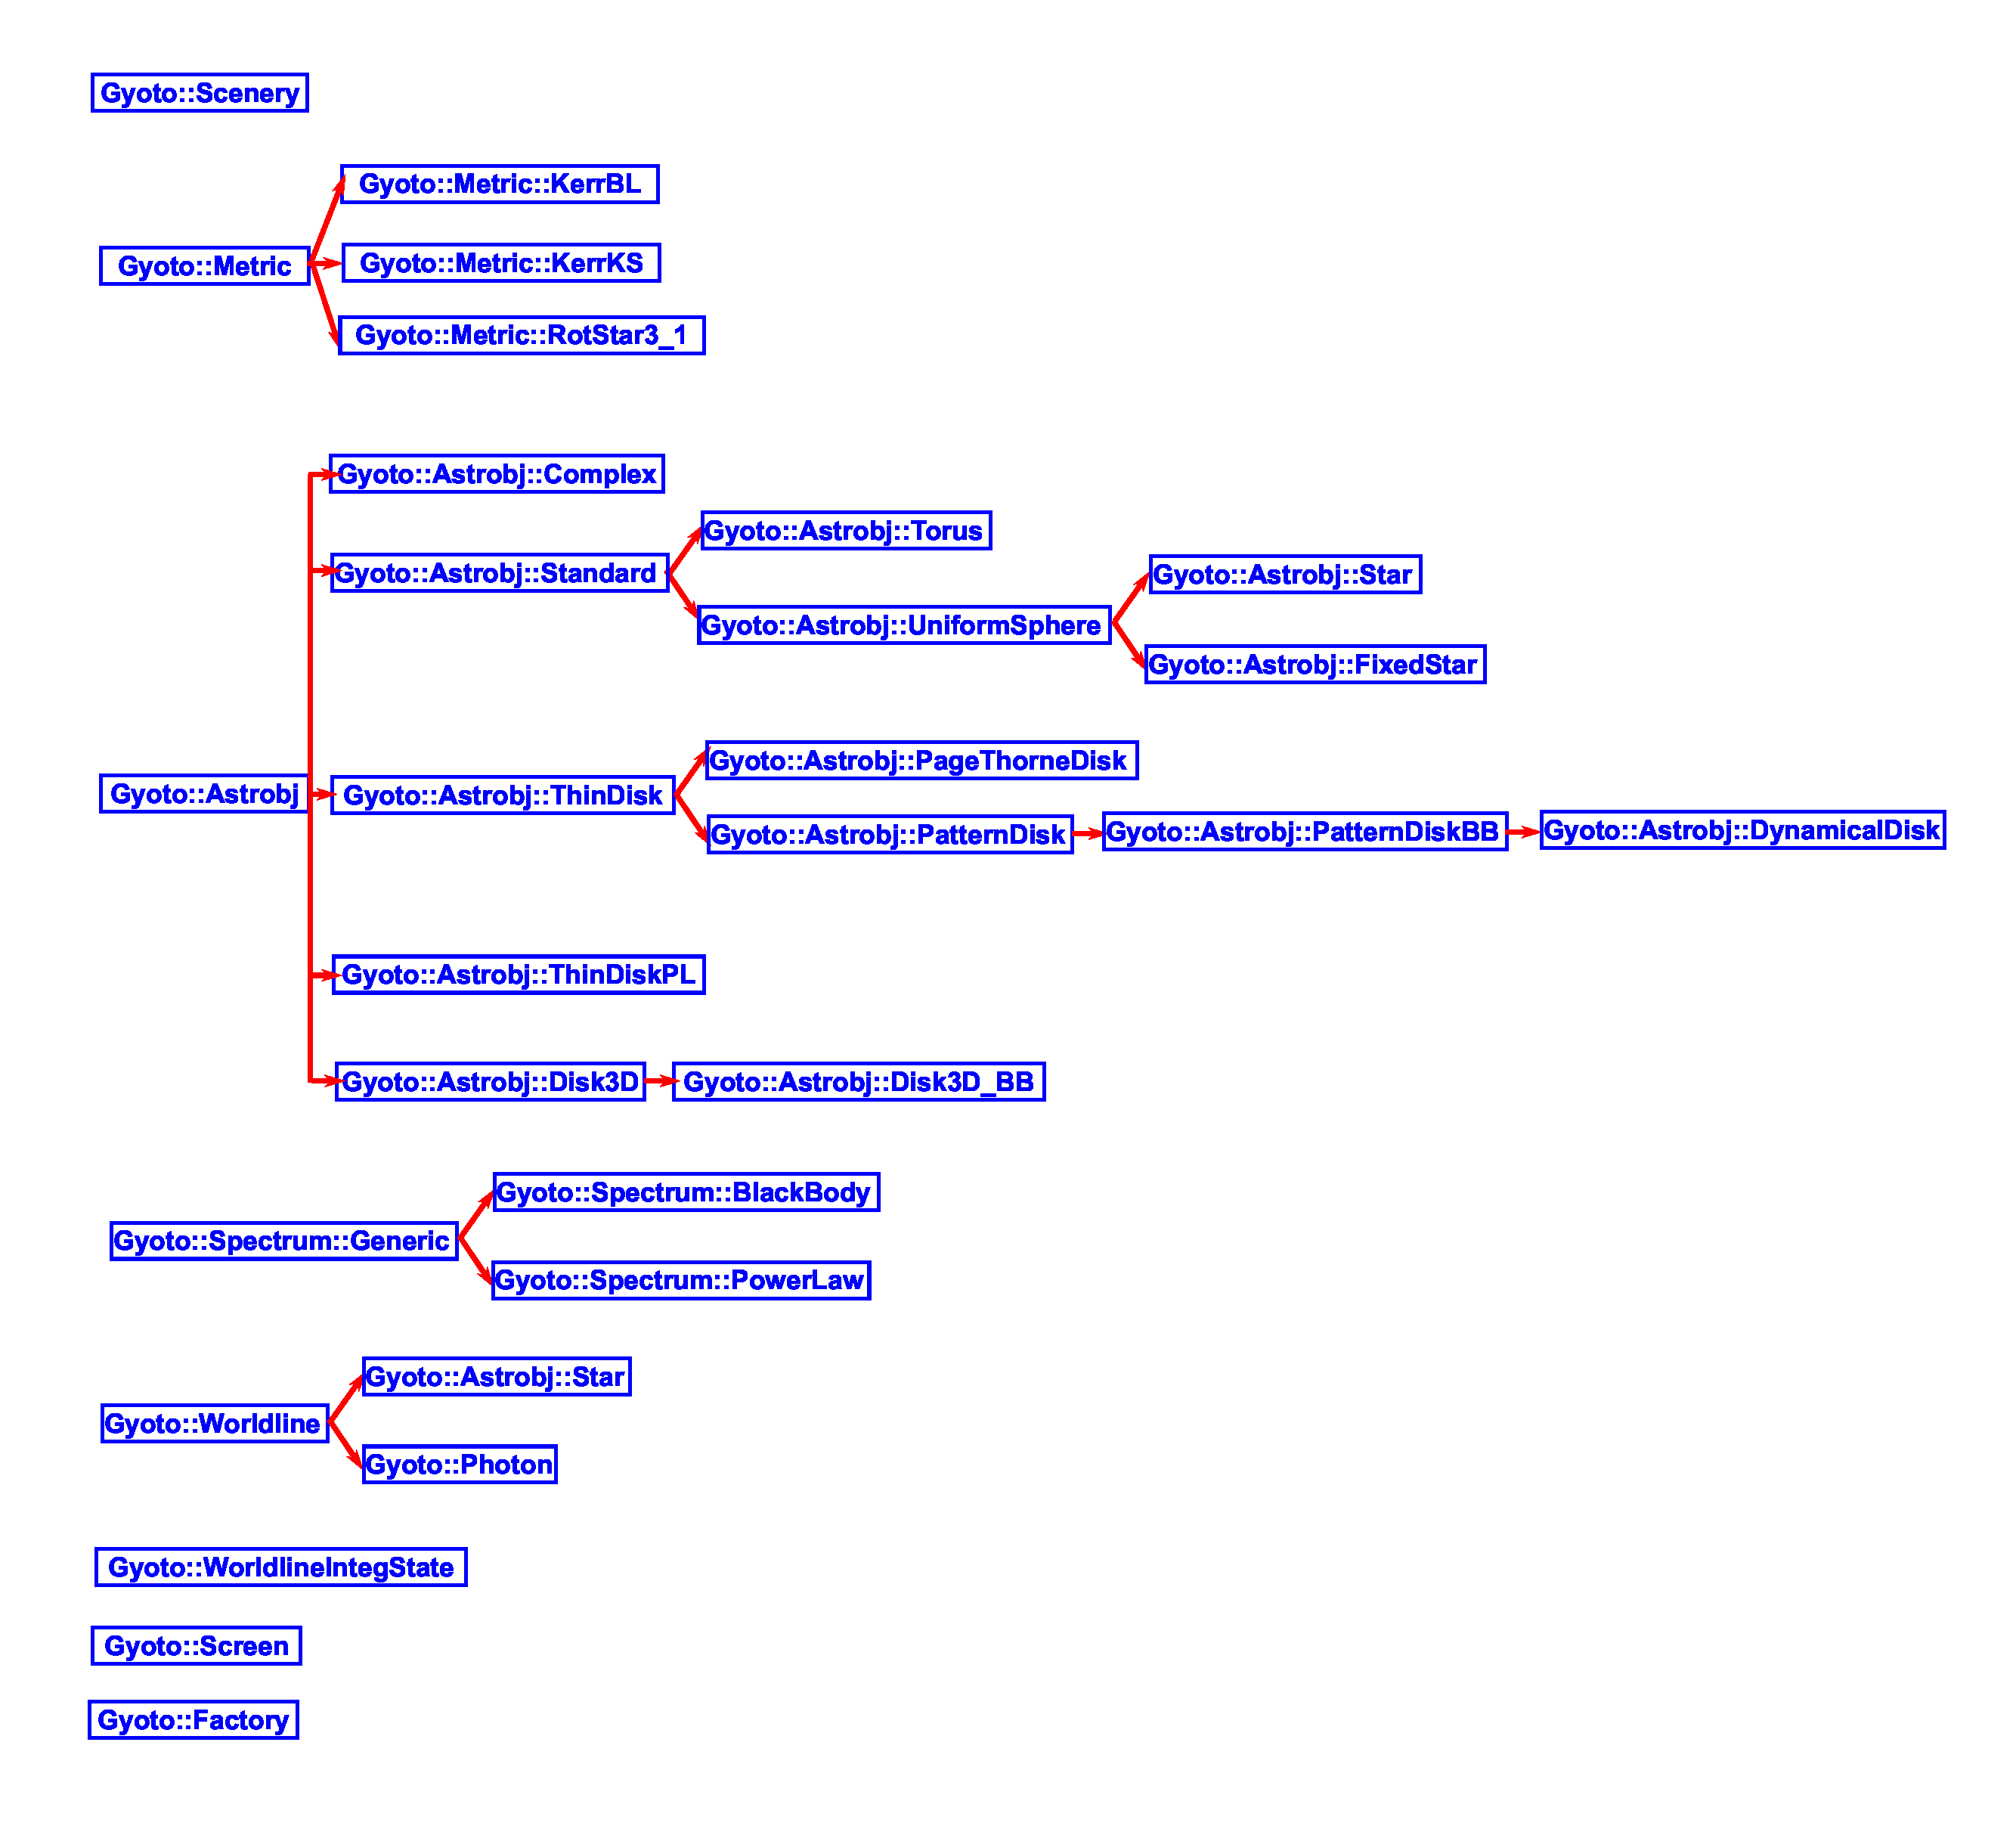
\includegraphics[width=18cm,height=20cm]{ClassHierarch.pdf}
\caption{Hierarchy of \texttt{GYOTO} C++ main classes.}
\label{fig:hierarch}
\end{figure}

\subsection{A typical \texttt{GYOTO} computation}

\begin{sloppypar} %to allow proper newline for long words (in texttt)
Let us now describe the main interactions of these various classes during the computation of one given photon, ray-traced in the Kerr metric in Boyer-Lindquist coordinates towards, for instance, a \texttt{PageThorneDisk}, i.e. a geometrically thin optically thick disk following \citet{page74}.

All directories used in the following are located in \texttt{GYOTO} home directory.

\texttt{GYOTO} \texttt{main} program is located in \texttt{bin/gyoto.C}. This program first interprets the command line given by the user. It creates a new \texttt{Factory} object, initialised by means of the \texttt{XML} input file, that will itself create (see \texttt{lib/Factory.C}) the \texttt{Scenery}, \texttt{Screen} and \texttt{Astrobj} objects. The output quantities the user is interested in (image, spectrum...) will be stored during the computation in the \texttt{data} object, of type \texttt{Astrobj::Properties}. The \texttt{Scenery} object is then used to perform the ray-tracing, by calling its \texttt{rayTrace} function. All the functions that begin with \texttt{fits\_} allow to store the final output quantities in \texttt{FITS} format.

The function \texttt{Scenery::rayTrace} calls \texttt{Photon::hit} that forms the core of \texttt{GYOTO}: \texttt{Photon::hit} integrates the null geodesic from the observer's screen backward in time until the target object is reached (there are other stop conditions of course, see \texttt{lib/Photon.C}). \texttt{Photon::hit} is basically made of a loop that calls the function \texttt{WorldlineIntegState::nextStep} until a stop condition is reached.  \texttt{WorldlineIntegState::nextStep} itself calls the correct adaptive fourth order Runge-Kutta integrator (RK4) , depending on the metric used. Here, the metric being \texttt{KerrBL}, the RK4 used is \texttt{KerrBL::myrk4\_adaptive}. 

Moreover, the \texttt{Photon::hit} also calls the \texttt{Astrobj::Impact} function that asks the \texttt{Astrobj} whether the integrated photon has reached it or not. When the photon has reached the target, this \texttt{Astrobj::Impact} function calls the \texttt{Astrobj::processHitQuantities} function that updates the \texttt{data} depending on the user's specifications. 
\end{sloppypar}

\section{Computing an image or a spectrum in the Kerr metric with \texttt{GYOTO}}
\label{kerr}

\subsection{The \texttt{Screen}}

The observer's \texttt{Screen} is made of $N\times N$ pixels, and has a field of view of $f$ radians. The field of view is defined as the maximum angle between the normal to the screen and the most tangential incoming geodesic. 

Keep in mind that the screen is point-like, the different pixels are all at the same position (the one and only screen position defined in the \texttt{XML} file), but the various pixels define various angles on the observer's sky.  For instance, if $f=\pi / 2$ (which gives a view of the complete half space in front of the screen), the geodesic that hits the screen on the central pixel $(i=N/2,j=N/2)$ comes from the direction normal to the screen whereas the geodesic that hits the screen on the $(i=N,j=N/2)$ pixel comes from a direction tangential to the screen.

Each pixel of the screen thus covers a small solid angle on the observer's sky. This elementary solid angle is equal to the solid angle subtended by a cone of opening angle $f$ divided by the number of pixels: $\delta\Omega_{\mathrm{pixel}} = 2\,\pi\,(1-\cos f) / N^{2}$ (assuming the field of view is small enough).

\subsection{Computing an image}

The quantity that is carried along the geodesics computed by \texttt{GYOTO} in most cases is the specific intensity $I_{\nu}$ ($\mathrm{erg\,cm^{-2}\,s^{-1}\,ster^{-1}\,Hz^{-1}}$).

An image is then defined as a map of specific intensity: each pixel of the screen contains one value of $I_{\nu}$, that can then be plotted. It is important to keep in mind that such an "image" is not physically equivalent to a real image that would be obtained with a telescope: a real image is a map of specific fluxes values, and a specific flux is the sum of the specific intensity on some solid angle.

An example of image computation has already been given in Section~\ref{demo}.


\subsection{Computing a spectrum}



To compute a spectrum, the \texttt{Screen} field of the \texttt{XML} file should contain information about the observed frequency range. For a real telescope, this means adding a spectrometer. The additional command in the \texttt{XML} file is thus:

\begin{code}
<Spectrometer kind="freqlog" nsamples="20">5. 25.</Spectrometer>
\end{code}

This line means that that $20$ values of observed frequencies will be considered, evenly spaced logarithmically, between $10^{5}$ and $10^{25}$ Hz. It is possible to choose frequencies linearly evenly spaced by using \texttt{freq} instead of \texttt{freqlog}. It is also possible to use wavelengths instead of frequencies, see \texttt{GyotoScreen.h} for more information.

Moreover, the \texttt{XML} file should explicitly state that the quantity of interest is no longer a simple image, but a spectrum. This is allowed by the following command, that should be added for instance before the end of \texttt{Scenery} field:

\begin{code}
<Quantities>Spectrum</Quantities>
\end{code}
When this command is used, the output \texttt{FITS} file will contain a cube of images, each image corresponding to one observed frequency.

Computing the spectrum is now straightforward. Remembering that the flux is linked to the intensity by:

\begin{equation}
\D F_{\nu_{\mathrm{obs}}} = I_{\nu_{\mathrm{obs}}}\,\cos\theta\,\D \Omega,
\end{equation}
where $\Omega$ is the solid angle under which the emitting element is seen, and $\theta$ is the angle between the normal to the observer's screen and the direction 
of incidence, the flux is given by:

\begin{equation}
\label{deffluxGyoto}
F_{\nu_{\mathrm{obs}}} = \sum_{\mathrm{pixels}} I_{\nu_{\mathrm{obs}},\mathrm{pixel}}\,\cos(\theta_{\mathrm{pixel}})\,\delta\Omega_{\mathrm{pixel}} ,
\end{equation}
where $I_{\nu_{\mathrm{obs}},\mathrm{pixel}}$ is the specific intensity reaching the given pixel, $\theta_{\mathrm{pixel}}$ is the angle between the normal to the screen and the direction of incidence corresponding to this pixel and $\delta\Omega_{\mathrm{pixel}}$ is the element of solid angle introduced above. 

This quantity $F_{\nu_{\mathrm{obs}}}$ can thus be very simply
computed from the cube of specific intensities computed by
\texttt{GYOTO}. Examples of spectra computed by \texttt{GYOTO} can be
found in, e.g.,~\citet{straub12}. Section~\ref{sect:yorick} contains
example code to compute a spectrum directly using the provided Yorick
interface. See also \texttt{yorick/check-polish-doughnut.i}, which
does just that as part of the routine test suite of \GYOTO.


\section{\texttt{GYOTO} in numerical metrics}
\label{3+1}

A specificity of \texttt{GYOTO} is its ability to ray-trace in non-Kerr metrics, numerically computed in the framework of the 3+1 formalism of general relativity~\citep{gourgoulhon12}, e.g. by means of the open source LORENE library developed by the Numerical Relativity group at Observatoire de Paris/LUTH\footnote{\url{http://www.lorene.obspm.fr/}}. 

\begin{sloppypar}
For the time being, only a simple example of numerical metric is implemented in the public version of \texttt{GYOTO}: the metric of a relativistic rotating star. The file \texttt{doc/examples/example-movingstar-rotstar3\_1.xml} allows to ray-trace a basic \texttt{GYOTO} moving \texttt{Star} in this metric. The file \texttt{resu.d} specified in the \texttt{XML} file is the output of a LORENE computation for the metric of a rotating relativistic star by the LORENE/nrotstar code.
\end{sloppypar}

The basic functions developed in \texttt{lib/RotStar3\_1.C} are similar to their Kerr counterparts, but here the metric is expressed in terms of the 3+1 quantities (lapse, shift, 3-metric, extrinsic curvature). The equation of geodesics expressed in the 3+1 formalism is given in~\citet{vincent12a} and implemented in \texttt{lib/RotStar3\_1.C}. However, it is possible to choose in the \texttt{XML} file whether the integration will be performed by using this 3+1 equation of geodesics, or by using the most general 4D equation of geodesics~\citep[see][for a comparison of the two methods]{vincent11a}.

\section{Local tetrads: setting the Screen orientation}

The orientation of the camera (implemented by the class
\texttt{Gyoto::Screen} in C++ and gyoto.core.Screen in Python) is
determined by a local tetrad of the observer composed of four 4-vectors
$(\vec u, \vec e_l, \vec e_u, \vec e_f)$ which form an orthonormal
local basis and where:
\begin{description}
\item[$\vec u$] is the 4-velocity of the observer;
\item[$\vec e_l$] points to the left-hand side of the observer;
\item[$\vec e_u$] points up;
\item[$\vec e_f$] points front, i.e. in the direction where the
  observer is looking.
\end{description}

In the following, $(\vec e_t, \vec e_r, \vec e_\theta, \vec
e_\varphi)$ is the usual spherical local basis, which can also be
defined for Cartesian coordinate systems $(t, x, y, z)$ such as
\texttt{KerrKS} as follows:
$$
\begin{array}{rcl}
  r & = & \sqrt{x^2+y^2+z^2} \\
  r_p & = & \sqrt{x^2+y^2} \\
  \theta & = & \atantwo(r_p, z) \\
  \varphi & = & \atantwo(y, x) \\
  \vec e_t & = & (1, 0, 0, 0) \\
  \vec e_r & = &  (0, x/r, y/e, z/r) \\
  \vec e_\theta & = &  (0, \cos \theta \cos \varphi, \cos \theta \sin\varphi, -\sin \theta)\\
  \vec e_\varphi & = & (0, -\sin \varphi, \cos \varphi, 0)  \\
\end{array}
$$


The Screen interface provides several ways to specify this tetrad with
the concept of \texttt{ObserverKind} (XML entity), which can be set
using the Screen method \texttt{observerKind()}:
\begin{description}
\item[\texttt{ObserverAtInfinity}] the default, does no special
  treatment, which implicitly assumes $(\vec u, \vec e_l, \vec e_u,
  \vec e_f) = (\vec e_t, -\vec e_\varphi, -\vec e_\theta, -\vec
  e_r)$. In this case, the Screen orientation can be fine-tuned using
  the XML entities \texttt{PALN}, \texttt{Dangle1} and
  \texttt{Dangle2}, corresponding to the methods \texttt{PALN()},
  \texttt{dangle1()} and \texttt{dangle2()}. This default is fine for
  most cases, i.e. when the observer really is far from the the
  central object (more than a few 10 geometrical units) and at rest.
\item[\texttt{ZAMO}] is the natural extension of
  \texttt{ObserverAtInfinity} in stronger field. $\vec u$ is first
  computed using the Metric method \texttt{zamoVelocity} which returns
  $\vec e_t$ projected in the hyperplane orthogonal to $\vec
  e_\varphi$ and then normalized. This is the velocity of a
  zero-angular-momentum observer. Then, the base $(\vec u, -\vec
  e_\theta, -\vec e_r, -\vec e_\varphi)$ is orthonormalized into
  $(\vec u, \vec e_u, \vec e_f, \vec e_l)$ using the Gram--Schmidt
  process as implemented in the Metric method
  \texttt{GramSchmidt}. The order of this orthonormalization matters
  to get the same tetrad as propsed by Krolik, Hawley \& Hirose (2005,
  ApJ:622:1008), implemented in \texttt{KerrBL}.
\item[\texttt{VelocitySpecified}] applies the same process but using a
  user-supplied, arbitrary 4-velocity using the XML entity
  \texttt{FourVel} or the Screen method \texttt{fourVel}.
\item[\texttt{FullySpecified}] is the most versatile, since the user
  provides the four vectors using the XML entities \texttt{FourVel}
  ($\vec u$), \texttt{ScreenVector1} ($\vec e_l$),
  \texttt{ScreenVector2} ($\vec e_u$) and \texttt{ScreenVector3}
  ($\vec e_f$) (the corresponding methods are the same, starting with
  first letter in lower case). The user is then responsible for
  providing a direct, orthonormal basis. For constructing this basis,
  the user can use the helper functions described below.
\end{description}

In the rest of this section, we will use the Python API to document
and demonstrate the use of the various helper methods that can be used
to construct a local tetrad. Those lines can be translated to C++ in a
trivial manner. Let \texttt{MetricKind} be a Metric kind
(e.g. \texttt{KerrBL}, \texttt{KerrKS} or other), \texttt{AstrobjKind}
be a kind of Astrobj, and $x0, x1, x2, x3$ be coordinates in this
Metric.
\begin{code}
  from gyoto import core
  import numpy
  from matplotlib import pyplot as plt

  metric=core.Metric('KerrBL')        # make and initialize a metric

  scr=core.Screen()                   # make a Screen
  scr.metric(metric)
  scr.resolution(32)
  scr.fieldOfView(60, 'degree')
  scr.anglekind('Rectilinear')

  ao=core.Astrobj('ThinDisk')         # make an astrobj,
  ao.metric(metric)                   # initialize it
  ao.set('InnerRadius', 6.)
  ao.rMax(200)

  sc=core.Scenery()                   # make Scenery
  sc.metric(metric)                   # assign metric
  sc.astrobj(ao)                      # assign astrobj
  sc.screen(scr)                      # assign screen
  
  x0, x1, x2, x3=0., 15., numpy.pi/4, numpy.pi/4
  pos=numpy.asarray([x0, x1, x2, x3]) # this is a 4 position
  scr.setObserverPos(pos)             # set observer position
  fourvel=numpy.zeros(4)              # NumPy array for 4-velocity
\end{code}

Now we can set the observer kind and ray-trace. The default would be:
\begin{code}
  scr.observerKind('ObserverAtInfinity')
  results=sc.rayTrace()
\end{code}
which will not work that close to the central object (15 geometrical
units in this example).

\begin{code}
  scr.observerKind('ZAMO')
  results=sc.rayTrace()
\end{code}
would always work, though. ZAMO stands for `zero angular momentum
observer'. One can display the intensity image:

\begin{code}
  plt.imshow(results['Intensity'], origin='bottom')
  plt.show()
\end{code}

To try \texttt{ObserverKind==VelocitySpecified}, we need to get a
4-velocity. Several methods can help with that (see for instance
\texttt{help(core.Metric.circularVelocity)}), but to continue with the
same example we shall retrieve the velocity of a ZAMO with:

\begin{code}
  metric.zamoVelocity(pos, fourvel)
\end{code}

Once the velocity vector has been set, one just needs to assign it to
the Screen:

\begin{code}
  scr.observerKind('VelocitySpecified')
  scr.fourVel(fourvel)
  results=sc.rayTrace()
  plt.imshow(results['Intensity'], origin='bottom')
  plt.show()
\end{code}

\texttt{zamoVelocity} is always defined. It provides a velocity with
zero angular momentum. \texttt{KerrBL.zamoVelocity} is an optimised
implementation, compatible with the generic one which projects $\vec
e_t$ on the hyperplane orthogonal to $\vec e_\varphi$. The same could
be implemented in Python like this:
\begin{code}
  ephi    = numpy.asarray([0., 0., 0., 1.])
  fourvel = numpy.asarray([1., 0., 0., 0.])

  if metric.coordKind()==core.GYOTO_COORDKIND_SPHERICAL:
      ephi    = numpy.asarray([0., 0., 0., 1.])
  else:
      phi=numpy.arctan2(pos[2], pos[1]);
      cp=numpy.cos(phi)
      sp=numpy.sin(phi)
      ephi=numpy.asarray([0., -sp, cp, 0.])

  metric.projectFourVect(pos, fourvel, ephi)
  metric.multiplyFourVect(fourvel, 1./abs(metric.norm(pos, fourvel)))
\end{code}

The snippet above has introduced three methods:
\begin{code}
  metric.multiplyFourVect(fourvel, scalar) 
\end{code}
just multiplies each element of fourvel by \texttt{scalar}. This C++
convenience method does the same as the more Pythonic:
\begin{code}
  fourvel *= scalar
\end{code}
where \texttt{fourvel} is a NumPy array and \texttt{scalar}
a... scalar. Likewise, for adding two vectors, this:
\begin{code}
  metric.addFourVect(fourvel, v)
\end{code}
is equivalent to this:
\begin{code}
  fourvel += v
\end{code}
where \texttt{fourvel} and \texttt{v} are two NumPy arrays of 4 elements.

\begin{code}
  metric.norm(pos, fourvel)
\end{code}
\texttt{norm} returns the norm of a 4-vector:
$\left\lVert\vec{v}\right\rVert=\sgn(\vec{v}\cdot\vec{v})\sqrt{\lvert\vec{v}\cdot\vec{v}\rvert}$. It
could also be computed as:
\begin{code}
  n2=metric.ScalarProd(pos, fourvel, fourvel)
  numpy.sign(n2)*numpy.sqrt(abs(n2))
\end{code}
where \texttt{ScalarProd} implements the scalar product.

\begin{code}
  metric.projectFourVect(pos, fourvel, ephi)
\end{code}
projects \texttt{fourvel} on the hyperplane orthogonal to
\texttt{ephi} and returns the projected vector in place. The
mathematical equivalent would be
$$\proj_{\vec v}(\vec u) = \vec u - \sgn(\lVert v\rVert) (\vec u \cdot \frac{\vec v}{\lvert \lVert \vec v \rVert \rvert}) \frac{\vec v}{\lvert \lVert \vec v \rVert \rvert}$$

\texttt{VelocitySpecified} instructs the Screen to build a local
tetrad for a camera looking towards the origin. The same can be done
with \texttt{FullySpecified} like this:

\begin{code}
  scr.observerKind('FullySpecified')
  el=numpy.zeros(4)
  eu=numpy.zeros(4)
  ef=numpy.zeros(4)
  metric.observerTetrad(pos, fourvel, el, eu, ef)
  scr.fourVel(fourvel)
  scr.screenVector1(el)
  scr.screenVector2(eu)
  scr.screenVector3(ef)
  results=sc.rayTrace()
  plt.imshow(results['Intensity'], origin='bottom')
  plt.show()
\end{code}

If \texttt{fourvel} has been set using
\texttt{metric.zamoVelocity(pos, fourvel)}, this actually is
equivalent to setting \texttt{ObserverKind} to \texttt{'ZAMO'}.

The method \texttt{gyoto.animate.orbiting\_screen\_forward} provides a
complete example where the local tetrad is computed in Python,
orthonormalized using \texttt{metric.GramSchmidt} and passed to the
Screen where the property \texttt{ObserverKind} has been set to
\texttt{FullySpecified}. We comment on a simplified version below.

The goal of this code is to set the camera such that it looks in the
direction where the Screen is moving, so $\vec e_f$ is initialized as
the 3-velocity $(0, \dot x^1 / \dot x^0, \dot x^2 / \dot x^0, \dot x^3
/ \dot x^0)$. $\vec e_u$ is initialized as $\proj_{e_f}(\vec e_r)$ and
normalized. It is therefore a vector pointing away from the central
object, orthogonal to $e_f$ and normal (in the 3D Euclidian sense). We
set $\vec e_l=\vec e_u \times \vec e_f$ where $\times$ denotes the 3D
external (vector) product. Thus, $(\vec e_l, \vec e_u, \vec e_f)$
would form an orthonormal basis of a Euclidian 3D space. We then use
the Gram--Schmidt process to orthonormalize the tetrad $(\vec u, \vec
e_u, \vec e_f, \vec e_l)$ in the metric sense. Most computations are
done in Cartesian 3D coordinates, for the sake of computing the
external product easily.

\begin{code}
  pos=numpy.asarray([x0, x1, x2, x3]) # this is a 4 position
  fourvel=numpy.zeros(4)
  metric.circularVelocity(pos, fourvel)

  # pos and fourvel have been initialized previously
  coord=numpy.concatenate((pos, fourvel))
  ef=numpy.zeros(4)
  # get Cartesian expression of 3-velocity into ef[1:]:
  metric.cartesianVelocity(coord, ef[1:])
  # normalize ef to 1 (in 3D):
  ef /= numpy.sqrt((ef*ef).sum())

  # get Cartesian expression of position in posc
  # as well as spherical radius in r:
  if metric.coordKind()==core.GYOTO_COORDKIND_SPHERICAL:
      t=pos[0]
      r=pos[1]
      theta=pos[2]
      phi=pos[3]
      st=numpy.sin(theta)
      ct=numpy.cos(theta)
      sp=numpy.sin(phi)
      cp=numpy.cos(phi)
      posc=[pos[0], r*st*cp, r*st*sp, r*ct]
  else:
      posc=pos
      r=numpy.sqrt(pos[1:]**2).sum()

  # Now initialize eu as er, but project it orthogonally to ef in 3D
  # and then normalize it:    
  eu=numpy.concatenate(([0.], posc[1:]/r))
  eu -= (ef*eu).sum()*ef
  eu /= numpy.sqrt((eu*eu).sum())

  # Last vector is el, which we construct as the 3D vector product
  # between eu and ef, computed in Cartesian coordinates:
  el=numpy.zeros(4)
  el[1]=eu[2]*ef[3]-eu[3]*ef[2]
  el[2]=eu[3]*ef[1]-eu[1]*ef[3]
  el[3]=eu[1]*ef[2]-eu[2]*ef[1]

  # If the coordinate system is spherical, we need to convert back:
  if metric.coordKind()==core.GYOTO_COORDKIND_SPHERICAL:
      er=posc/r
      ephi=numpy.asarray([0., -sp, cp, 0.])
      etheta=numpy.asarray([0., ct*cp, ct*sp, -st])
      ef=numpy.asarray([
        0.,
        (er*ef).sum(),
        (etheta*ef).sum(),
        (ephi*ef).sum()
      ])
      eu=numpy.asarray([
        0.,
        (er*eu).sum(),
        (etheta*eu).sum(),
        (ephi*eu).sum()
      ])
      el=numpy.asarray([
        0.,
        (er*el).sum(),
        (etheta*el).sum(),
        (ephi*el).sum()
      ])

  # Our 3 vectors form an orthonormal basis in the Euclidian sense,
  # but the tetrad still needs to be orthonormalized in the metric
  # sense:
  metric.GramSchmidt(pos, fourvel, eu, ef, el);

  # Then we just need to attach the tetrad to the Screen:
  scr.observerKind('FullySpecified')
  scr.setObserverPos(pos)
  scr.fourVel(fourvel)
  scr.screenVector1(el)
  scr.screenVector2(eu)
  scr.screenVector3(ef)

  # Perform ray-tracing as usual:
  results=sc.rayTrace()
  plt.imshow(results['Intensity'], origin='bottom')
  plt.show()
 
\end{code}

\section{Extending \GYOTO}

This section is currently under construction.

\GYOTO\ can be extended easily by adding new \Metric, \Astrobj, and
\Spectrum\ classes. Such classes can be written in the Python language
(Sect.~\ref{sect:python-plug-in}) or in C++, in which case they are made
available to Gyoto by cumpiling them into a \GYOTO\ plug-in
(Sect.~\ref{sect:plug-in}). The main \GYOTO\ code-base already contain
tree plug-ins:
\begin{itemize}
\item \texttt{stdplug}, which contain all the standard analytical
  metrics and all the standard astrophysical object;
\item \texttt{python}, which allows implementing new \Metric,
  \Astrobj, and \Spectrum\ classes in the Python (2 or 3) language;
\item and \texttt{lorene}, which contains the numerical, LORENE-based
  metrics.
\end{itemize}
In addition, we maintain our own private plug-in, which contains
experimental or yet unpublished \Astrobj\ and \Metric\ classes. When
we make a publication based on these classes, we try to move them from
our private plug-in to the relevant public plug-in. We kindly request
that you follow the same philosophy: whenever you write a new class
and make a publication out of it, please publish the code as free
software, either on your own servers or by letting us include it in
\GYOTO.

As soon as you write your own objects (especially if you do so in
C++), you will dependent on the stability of the \GYOTO\ application
programming interface, which is subject to frequent changes. It will
help us to help you maintain your code if you inform us of such
development: \texttt{gyoto@sympa.obspm.fr}. In addition, we try to
maintain a stable branch in our github repository
(\url{http://github.com/gyoto/Gyoto}). Code on this branch should
remain API-and ABI-compatible with the latest official release.

\subsection{Extending in Python}
\label{sect:python-plug-in}
The `python' plug-in allows writting derived classes
in Python rather than C++.

This is the easiest approach and lets you set-up your new
objects in just a few lines of code, without the need for setting-up a
plug-in, compiling it frequently during your deverlopment
cycle. However, there is a cost in terms of code execution speed. This
code is usually negligible to moderate for classes implementing the
\Astrobj\ and \Spectrum\ interfaces, but it is major for classes
implementing the \Metric\ interface. This is because the \Metric\
methods are evaluated several times per iteration when iterating
geodesics, while the \Astrobj\ and \Spectrum\ methods are evaluated
less frequently.

To use your Python classes, simply load the Python plug-in, for
instance by setting the \texttt{GYOTO\_PLUGINS} environment variable
to include the ``python''\footnote{The actual name of the Gyoto plug-in
  will match that of the Python interpreter used for compiling it. For
  instance, if Gyoto was configured with \texttt{./configure
    PYTHON=/usr/bin/python3.4}, the plug-in will be called
  \texttt{python3.4} instead of \texttt{python}. This allows you to
  compile several versions of the plug-in, that will run inside each
  of the Python interpreters.} plug-in (see
Sect.~\ref{sect:using-plug-in}). Then tell the plug-in about your
module and class. For instance, in an XML file:
\begin{code}
  <Metric kind="Python">
   Python module name for ``my_module.py'':
    <Module>my_module</Module>

   Class defined in ``my_module.py'':
    <Class>my_class</Class>

   Any parameters (foating point) ``my_class'' may need:
    <Parameters>2.0 20.0</Parameters>
  </Metric>
\end{code}

The Python class will need to implement a few methods, with the same
name as the C++ method it implements (except the C++ name
\texttt{operator()} is translated as \texttt{\_\_call\_\_} in Python).

More information can be found in the doxygen-generated documentation
for the
\href{https://github.com/gyoto/Gyoto/blob/master/plugins/python/include/GyotoPython.h}{\texttt{GyotoPython.h}}
file and in the
\href{https://github.com/gyoto/Gyoto/tree/master/plugins/python/doc/examples}{\texttt{plugins/python/doc/examples}}
sub-directory of the source code distribution.

\subsection{Writing a C++ plug-in}
\label{sect:plug-in}

A plug-in is merely a shared library which contains the object code
for your new objects, plus a special initialisation function. It is
loaded into memory using \texttt{dlopen()} by the function
\texttt{Gyoto::loadPlugin(char const*const name, int nofail)} (note
that the upper level function \texttt{Gyoto::requirePlugin(char
  const*const name, int nofail)} should be used instead whenever
applicable), implemented in \texttt{lib/Register.C}. The \texttt{name}
argument will be used three times:
\begin{itemize}
\item the shared library file must be called
  \texttt{libgyoto-\emph{name}.\$suffix} (\texttt{\$suffix} is usually
  \texttt{.so} under Linux, \texttt{.dylib} under Mac OS);
\item the init function for your plug-in must be called either
  \texttt{\_\_Gyoto\emph{name}Init} or exactly
  \texttt{\_\_GyotoPluginInit};
\item each subcontractor registered by the init function (see below)
  will be tagged with the plug-in name, so it is later possible to
  search for a registered subcontractor by kind name and plugin name.
\end{itemize}

The role of the init function is to register subcontractors for your
object classes so that they can be found by name. For instance,
assuming you want to bundle the Minkowski metric (actually provided in
the standard plug-in) in a plugin called \texttt{myplugin}, you would
write a C++ file (whose name is not relevant, but assume
\texttt{MyPlugin.C}) with this content:

\begin{code}
#include "GyotoMinkowski.h"
using namespace Gyoto;
extern "C" void __GyotomypluginInit() {
  Metric::Register("Minkowski", \&Metric::Subcontractor<Metric::Minkowski>);
}
\end{code}

Likewise, you could register more metrics, astrophysical objects and
spectra. Other examples can be seen in the \texttt{lib/StdPlug.C} and
\texttt{lib/LorenePlug.C} files, and in the \texttt{plugins/python/}
directory.

When building your plug-in, make sure \texttt{MyPlugin.C} ends up
compiled with\\ \texttt{lib/Minkowski.C} (in this example) into a
single shared library called\\ \texttt{libgyoto-myplugin.so} (assuming
you work under Linux), and drop this file somewhere where Gyoto
will find it at run-time. Gyoto will try to ldopen the plug-ins from
the following locations in order (some variables are defined in
\texttt{gyoto.pc}, see below):
\begin{itemize}
\item wherever the run-time linker looks by default, which typically
  includes:
  \begin{itemize}
  \item any directory listed in the \texttt{\$LD\_LIBRARY\_PATH}
    environment variable;
  \item \texttt{/usr/local/lib/};
  \item \texttt{/usr/lib/};
  \end{itemize}
\item \texttt{\$\{localpkglibdir\}/\$\{GYOTO\_SOVERS\}/};
\item \texttt{\$\{localpkglibdir\}/} (typically \texttt{/usr/local/lib/gyoto});
\item \texttt{\$\{GYOTO\_PLUGDIR\}/}, this is the directory where the
  standard plug-ins shipped with Gyoto are installed (typically
  \texttt{\$\{pkglibdir\}/\$\{GYOTO\_SOVERS\}/});
\item \texttt{\$\{pkglibdir\}/} (typically
  \texttt{/usr/local/lib/gyoto} or \texttt{/usr/lib/gyoto}).
\end{itemize}
Note that \texttt{\$\{localpkglibdir\}} is defined only when it makes
sense (i.e. when Gyoto is not itself installed under \texttt{/usr/local}).

\GYOTO\ ships a pkg-config file (\texttt{gyoto.pc}) which stores
useful build-time information such as the install prefix and the
plug-in suffix. This file gets installed in the standard location, by
default \texttt{/usr/local/lib/pkgconfig/gyoto.pc}.

The Gyoto source code contains several examples of plug-ins. One of
them is minimalistic and its only purpose is to illustrate how to
build a plug-in, including an autoconf-based build system that parses
\texttt{gyoto.pc}. It is a good starting point for writing your own
plug-in. See the content of the subdirectory \texttt{plugins/null/},
in particular the \texttt{README} file.

\subsection{Adding a new metric (\Metric)}

The simplest example for a \Metric\ object is certainly the
\texttt{Minkowski} class. Let's go through the header file that
defines its interface (expunged from all this useless documentation
\texttt{;-)}), we trust the reader to go see the corresponding
\texttt{.C} file:\\
Avoid multiple and recursive inclusion of header files:
\begin{code}
  #ifndef __GyotoMinkowski_H_
  #define __GyotoMinkowski_H_
\end{code}
Minkowski is a metric, include the \Metric\ base class header file:
\begin{code}
  #include <GyotoMetric.h>
\end{code}
Declare that our new class goes into the \texttt{Gyoto::Metric}
namespace:
\begin{code}
  namespace Gyoto {
    namespace Metric { class Minkowski; }
  }
\end{code}
Declare that Minkowski inherits from the base class:
\begin{code}
  class Gyoto::Metric::Minkowski
  : public Gyoto::Metric::Generic
  {
\end{code}
Each class must be friend with the corresponding \texttt{SmartPointer}
class:
\begin{code}
    friend class Gyoto::SmartPointer<Gyoto::Metric::Minkowski>;
\end{code}
Minkowski has no private data, else we would put it here:
\begin{code}
    private:

\end{code}
Every class needs a constructor, which will at least populate the
\texttt{kind\_} attribute of the parent class and the kind of coordinate
system (Cartesian-like or spherical-like):
\begin{code}
  public:
    Minkowski();
\end{code}
The cloner is important, and easy to implement. It must provide a deep
copy of an object instance. It is used in the multi-threading case to
make sure two threads don't tip on each-other's toes, and in the
Yorick plug-in (Sect.~\ref{sect:yorick}) when you want to make a copy
of an object rather than reference the same object:
\begin{code}
    virtual Minkowski* clone() const ;
\end{code}
Then come the two most important methods, which actually define the
mathematical metric:
\begin{code}
  void gmunu(double g[4][4], const double * x) const ;
  int christoffel(double dst[4][4][4], const double * x) const ;
\end{code}
The \texttt{setParameter} method is the one that interprets options
from the XML file. For each XML entity found in the \Metric\ section
in the form\\
\texttt{<ParName unit="unit\_name">ParValueString</ParName>},\\
 the method
\texttt{Metric::Generic::setParameters()} will call\\
\texttt{setParameter(ParName, ParValueString, unit\_name)}:
\begin{code}
    virtual void setParameter(std::string, std::string, std::string);
\end{code}
\texttt{setParameter()} should interpret the parameters specific to
this class and pass whatever remains to the \texttt{Generic}
implementation. \texttt{setParameter()} has a counterpart,\\
\texttt{fillElement()}, which is mostly used by the Yorick plug-in
(Sect.~\ref{sect:yorick}) to dump an in-memory object instance to text
format (this is what allows \texttt{gyotoy}, Sect.~\ref{sect:gyotoy},
to write its parameters to disk). This method must be compiled only if
XML input/output is compiled in:
\begin{code}
  #ifdef GYOTO_USE_XERCES
    virtual void fillElement(FactoryMessenger *fmp);
  #endif
\end{code}
The Minkowski implementation goes on with an alternate implementation
of \texttt{gmunu()} and \texttt{christoffel()}. For the purpose of
this documentation, we will skip these additional examples and close
the header file here:
\begin{code}
  };
  #endif
\end{code}

For more details, see the \GYOTO\ reference manual in
\texttt{doc/html/} or at \url{http://gyoto.obspm.fr/}. There are a few
other methods that are worthwhile reimplementing, such as
\texttt{circularVelocity()}, which allows getting accurate beaming
effects for thin disks and tori. Naturally,
\texttt{circularVelocity()} can only be implemented if circular orbits
physically exist in this metric (else, the Keplerian approximation is
readily provided by the generic implementation). Some other low-level
methods can be reimplemented, but it is not necessarily a good idea.

Once you have implemented the new Metric, just make sure it is
compiled into your plug-in and initialised in the initialisation
function (Sect.~\ref{sect:plug-in}). For official \GYOTO\ code (that
does not depend on LORENE), this is done by adding your \texttt{.C}
file to\\
\texttt{libgyoto\_stdplug\_la\_SOURCES} in
\texttt{lib/Makefile.am} (and running \texttt{autoreconf} followed by
\texttt{configure}), and adding one line in
\texttt{\_\_GyotostdplugInit} in \texttt{lib/StdPlug.C}.

\subsection{Adding a new spectrum (\Spectrum)}

Adding a new spectrum kind is almost the same as adding a metric.

\subsection{Adding a new astrophysical target object (\Astrobj)}
\label{newastrobj}

Adding a new astronomical object kind is almost the same as adding a
metric. However, astronomical objects are more complex than metrics
(they can have abundant hair). Instead of inheriting directly from the
most generic base class, \texttt{Gyoto::Astrobj::Generic}, you will
save yourself a lot of effort if you are able to derive from one of
the higher level bases:
\begin{description}
\item[Astrobj::ThinDisk] a geometrically thin disk
  (e.g. \texttt{PageThorneDisk}, \texttt{PatternDisk});
\item[Astrobj::UniformSphere] a... uniform sphere (e.g. \texttt{Star},
  \texttt{FixedStar});
\item[Astrobj::Standard] any object whose boundary can be defined as
  an iso-surface of some function of the coordinates, such as a sphere
  or a torus (e.g. \texttt{UniformSphere}, \texttt{Torus}).
\end{description}

\subsection{Using your new plug-in}
\label{sect:using-plug-in}
There are several ways to instruct \GYOTO\ to load your plug-in. You
can set the environment variable\texttt{GYOTO\_PLUGINS}\footnote{How
  to do it depends on your shell and is outside the scope of this
  manual.}, with a command such as
\begin{code}
  export GYOTO_PLUGINS=stdplug,myplugin
\end{code}
Alternatively, a list of plug-ins can be specified on the command-line
when using the \texttt{gyoto} tool:
\begin{code}
  $ gyoto --plugins=stdplug,myplugin ...
  $ gyoto -pstdplug,myplugin ...
\end{code}
%$
A plug-in can also be specified in the input XML file for each
section:
\begin{code}
   <Metric kind = "KerrBL" plugin="stdplug">
\end{code}
Finally, the Yorick interface (Sect.~\ref{sect:yorick}) has a function
to explicitly load a \GYOTO\ plug-in at run-time:
\begin{code}
 > gyoto.requirePlugin("myplugin");
\end{code}
Once the plug-in is loaded, your new object kinds should be registered
(that's the purpose of the init function). To check that your objects
are correctly register, you can use the \texttt{-{}-list} (or
\texttt{-l}) option of the \texttt{gyoto} tool or the
\texttt{gyoto.listRegister()} function of the Yorick interface:
\begin{code}
  $ gyoto --list [input.xml]
  $ gyoto -l [input.xml]
\end{code}
%$

You can use then use your classes directly in an XML file, using the
name you provided to the \texttt{Register()} function in the init
function of the plug-in:
\begin{code}
   <Metric kind = "Minkowski" plugin="myplugin">
\end{code}
The Yorick interface can load any object from an XML description, an
can also initialise any object from its name:
\begin{code}
 > metric = gyoto.Metric("Minkowski", "myplugin");
\end{code}
If your object supports any options using the \texttt{setParameter()}
method, these options can also be set from within Yorick:
\begin{code}
 > metric, setparameter="ParName", "ParValueString", unit="unit_string";
\end{code}
If your want finer access to your objects from the Yorick interface,
you will need to provide a Yorick plug-in around your \GYOTO\
plug-in. Look at the content of the \texttt{yorick/stdplug/}
directory. For new official \GYOTO\ objects in the standard plug-in,
it is fairly easy to provide an interface directly inside our Yorick
plug-in.

\subsection{Quality assurance}

It is customary to provide a test-suite for every new class in
\GYOTO. This normally includes an example file in
\texttt{doc/examples}, which is ray-traced in the \texttt{check}
target of \texttt{bin/Makefile.am}. Usually, we also provide a new
Yorick test file called\\
\texttt{yorick/check-myclass.i} which is
called from \texttt{yorick/check.i}. This is a good idea to do so even
if you don't intend on using the Yorick plug-in: at least, you can use
this interpreted interface to perform unit tests on your code in a
more fine-grained manner than a full-featured ray-traced image.

\bibliographystyle{kluwer}
\bibliography{\GyotoSrcDir/doc/user_guide/GyotoManual}


\end{document}

%%%Local Variables:
%%% mode: latex
%%% coding: utf-8
%%% TeX-PDF-mode: t
%%% ispell-local-dictionary: "en_GB"
%%%End:
